\section{Casos de Uso del Usuario}

\subsection{Diagrama de Casos de Uso General del Usuario}

\begin{figure}[htbp]
	\centering
		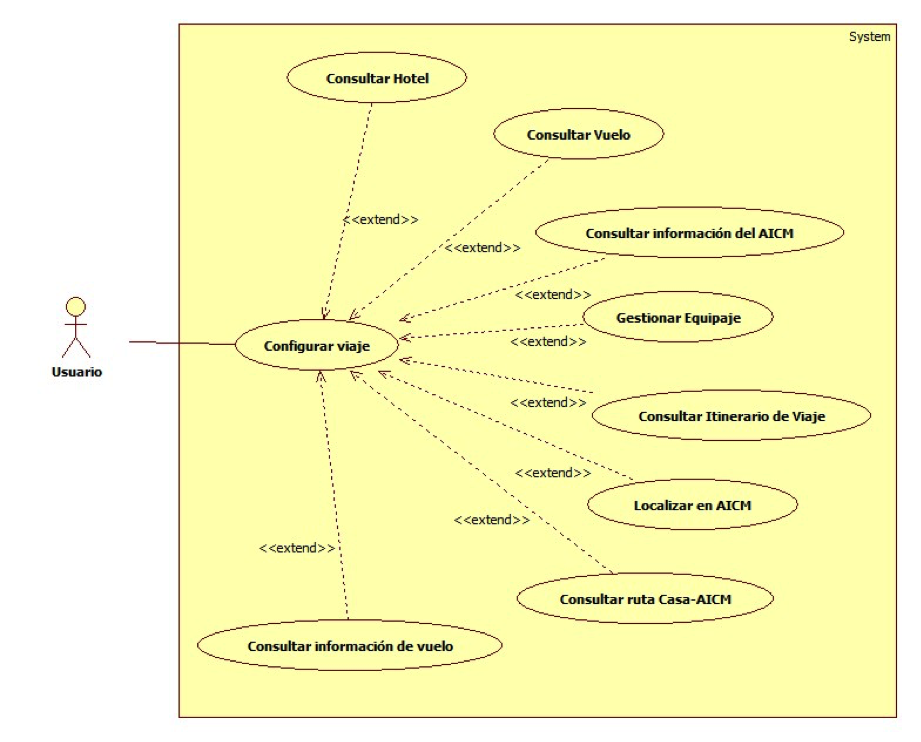
\includegraphics[width=0.9\textwidth]{Figuras/cugeneralUsuario.png}
		\rule{30em}{0.5pt}
	\caption[Diagrama de Casos de Uso General del Usuario]{Diagrama de Casos de Uso General del Usuario}
	\label{fig:cuGeneralUsuario}
\end{figure}

\subsection{Caso de Uso Configurar Viaje}

\begin{figure}[htbp]
	\centering
		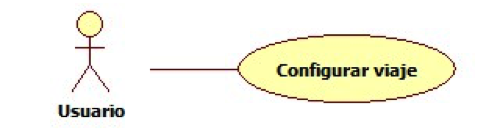
\includegraphics[width=0.9\textwidth]{Figuras/cuConfigurarViaje.png}
		\rule{30em}{0.5pt}
	\caption[Diagrama de Caso de Uso Configurar Viaje]{Diagrama de Caso de Uso Configurar Viaje}
	\label{fig:cuConfigurarViaje}
\end{figure}

\begin{longtable}[h]{|p{2.5cm}|p{6.4cm}|p{2cm}|p{2cm}|}
	\hline
		\rowcolor[RGB]{51,153,255}{Caso de Uso}&\multicolumn{2}{c}{Configurar Viaje}&{\textbf{CU-U-01}}\\
	\hline
		{Actores}&\multicolumn{3}{p{11.2cm}|}{Usuario}\\
	\hline
		{Tipo}&\multicolumn{3}{p{11.2cm}|}{Esencial}\\
	\hline
		{Precondición}&\multicolumn{3}{p{11.2cm}|}{El usuario puede o no realizar su configuración de viaje, pero la aplicación le hará la sugerencia de realizarla en otro momento.}\\
	\hline
		{Postcondición}&\multicolumn{3}{p{11.2cm}|}{La configuración del usuario ha quedado registrada, por lo tanto, está en condiciones de hacer uso de los servicios ofrecidos por el sistema.}\\
	\hline
		{Autor}&{Vivanco Carmona Erick Rafael}&{\textbf{Fecha} 09/01/15}&{\textbf{Versión} 2.0}\\
			\hline
		{Evaluador}&{Barajas Uribe Sergio}&{\textbf{Fecha} 15/01/15}&{\textbf{Estatus} Aprobado}\\
	\hline
		{Propósito}&\multicolumn{3}{p{11.2cm}|}{Configurar sus viajes dependiendo de la clase de viaje que más le agrade al usuario y la categoría de hoteles que frecuenta.}\\
	\hline
		{Resumen}&\multicolumn{3}{p{11.2cm}|}{El usuario realiza la configuración de la aplicación según la clase en la que más le gusta viajar y la categoría de hoteles que desea el usuario además proporciona su correo electrónico para tener el control de su usuario.}\\	
	\hline
		{Comentarios}&\multicolumn{3}{p{11.2cm}|}{Los datos guardados estarán protegidos y únicamente se enviaran notificaciones acerca de la aplicación al correo proporcionado.}\\	
	\hline
	\caption[Especificación del Caso de Uso Configurar Viaje]{Especificación del Caso de Uso Configurar Viaje}
    	\label{tab:cuConfigurarViaje}
\end{longtable}
\newpage
\begin{flushleft}
	\textbf{Trayectoria Principal}\\
	\begin{enumerate}
		\item El usuario inicia la aplicación por primera vez e inmediatamente se le indica si gusta configurar su aplicación con la clase en la que le guste viajar y categoría de hotel que prefiere. \hyperlink{TrayectoriaA_CU-U-01}{[Trayectoria A]}.
		\item El sistema presenta un formulario para que el usuario introduzca su correo electrónico, la clase de viaje y categoría de hotel.
		\item El usuario introduce los datos y los envía para que sean registrados.
		\item El sistema válida la configuración proporcionada por el usuario. \hyperlink{TrayectoriaB_CU-U-01}{[Trayectoria B]}.
		\item La configuración del usuario queda registrada en el sistema. Se notifica al usuario.
	\end{enumerate}
\end{flushleft}
----Fin del caso de uso

\begin{flushleft}
	\hypertarget{TrayectoriaA_CU-U-01}{}
	\textbf{Trayectoria Alternativa A}\\
	\textbf{Condición:} La conexión con el servidor se pierde. \\
	\textbf{Nota: } Este curso alterno puede presentarse en cualquier momento durante el curso de CU-U-01.\\
	\begin{enumerate}
		\item El cliente debe reintentar completar la operación en otro momento. 
		\item Volver a 1. 
	\end{enumerate}
\end{flushleft}
----Fin de Trayectoria

\begin{flushleft}
	\hypertarget{TrayectoriaB_CU-U-01}{}
	\textbf{Trayectoria Alternativa B}\\
	\textbf{Condición:} La configuración no es correcta.  \\
	\begin{enumerate}
		\item Se notifica al usuario y se solicita que los datos erróneos sean modificados. 
		\item Volver a 2.
	\end{enumerate}
\end{flushleft}
----Fin de Trayectoria
\newpage
\subsection{Caso de Uso Consultar Hotel}

\begin{figure}[htbp]
	\centering
		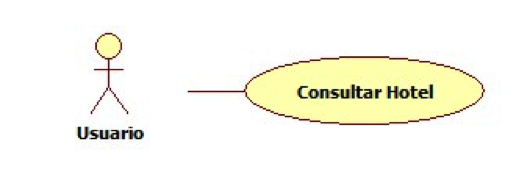
\includegraphics[width=0.9\textwidth]{Figuras/cuConsultarHotel.png}
		\rule{30em}{0.5pt}
	\caption[Diagrama de Caso de Uso Consultar Hotel]{Diagrama de Caso de Uso Consultar Hotel}
	\label{fig:cuConsultarHotel}
\end{figure}

\begin{longtable}{|p{2.5cm}|p{6.4cm}|p{2cm}|p{2cm}|}
	\hline
		\rowcolor[RGB]{51,153,255}{Caso de Uso}&\multicolumn{2}{c}{Consultar Hotel}&{\textbf{CU-U-02}}\\
	\hline
		{Actores}&\multicolumn{3}{p{11.2cm}|}{Usuario}\\
	\hline
		{Tipo}&\multicolumn{3}{p{11.2cm}|}{Esencial}\\
	\hline
		{Precondición}&\multicolumn{3}{p{11.2cm}|}{	Existen hoteles registrados en el Web Service.}\\
	\hline
		{Postcondición}&\multicolumn{3}{p{11.2cm}|}{El turista tiene a su disposición la información de hoteles acorde a sus posibilidades.}\\
	\hline
		{Autor}&{Vivanco Carmona Erick Rafael}&{\textbf{Fecha} 09/01/15}&{\textbf{Versión} 2.0}\\
			\hline
		{Evaluador}&{Barajas Uribe Sergio}&{\textbf{Fecha} 15/01/15}&{\textbf{Estatus} Aprobado}\\
	\hline
		{Propósito}&\multicolumn{3}{p{11.2cm}|}{Consultar información de hoteles.}\\
	\hline
		{Resumen}&\multicolumn{3}{p{11.2cm}|}{El usuario realiza una búsqueda de hoteles y se muestra un listado de los mismos según los parámetros de la búsqueda. }\\	
	\hline
	\caption[Especificación del Caso de Uso Consultar Hotel]{Especificación del Caso de Uso Consultar Hotel}
    	\label{tab:cuConsultarHotel}
\end{longtable}

\begin{flushleft}
	\textbf{Trayectoria Principal}\\
	\begin{enumerate}
		\item El usuario solicita consultar hoteles. \hyperlink{TrayectoriaA_CU-U-02}{[Trayectoria A]}.
		\item Se despliega un formulario para realizar la búsqueda según: ubicación del hotel o categoría del hotel.
		\item El usuario ingresa los parámetros de interés. \hyperlink{TrayectoriaB_CU-U-02}{[Trayectoria B]}.
		\item Se  muestra un listado de hoteles disponibles con las características requeridas. \hyperlink{TrayectoriaC_CU-U-02}{[Trayectoria C]}.
		\item El usuario puede realizar un filtrado de la lista por: estrellas de 1 a 5 o de 5 a 1; precios de bajo a alto o precios de alto a bajo.
		\item El usuario puede visualizar la información detallada de cada hotel.
	\end{enumerate}
\end{flushleft}
----Fin del caso de uso

\begin{flushleft}
	\hypertarget{TrayectoriaA_CU-U-02}{}
	\textbf{Trayectoria Alternativa A}\\
	\textbf{Condición:} La conexión con el servidor se pierde. \\
	\textbf{Nota: } Este curso alterno puede presentarse en cualquier momento durante el curso de CU-U-02. \\	
	\begin{enumerate}
		\item El cliente debe reintentar completar la operación en otro momento. 
		\item Volver a 1. 
	\end{enumerate}
\end{flushleft}
----Fin de Trayectoria

\begin{flushleft}
	\hypertarget{TrayectoriaB_CU-U-02}{}
	\textbf{Trayectoria Alternativa B}\\
	\textbf{Condición:} El usuario no ha ingresado los parámetros adecuados para la búsqueda. \\
	\begin{enumerate}
		\item  Se notifica al usuario y se solicita que indique los parámetros adecuados para la búsqueda.
	\end{enumerate}
\end{flushleft}
----Fin de Trayectoria

\begin{flushleft}
	\hypertarget{TrayectoriaC_CU-U-02}{}
	\textbf{Trayectoria Alternativa C}\\
	\textbf{Condición:} La búsqueda no obtiene resultados con las características requeridas. \\
	\begin{enumerate}
		\item Se despliega una notificación de aviso y se solicita iniciar una nueva búsqueda. 
		\item Volver a 1.
	\end{enumerate}
\end{flushleft}
----Fin de Trayectoria
\newpage
\subsection{Caso de Uso Consultar Vuelo}

\begin{figure}[htbp]
	\centering
		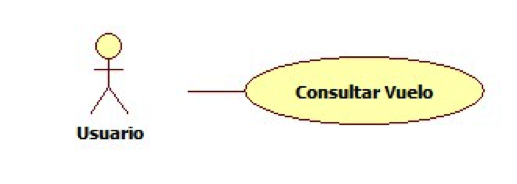
\includegraphics[width=0.9\textwidth]{Figuras/cuConsultarVuelo.png}
		\rule{30em}{0.5pt}
	\caption[Diagrama de Caso de Uso Consultar Vuelo]{Diagrama de Caso de Uso Consultar Vuelo}
	\label{fig:cuConsultarVuelo}
\end{figure}

\begin{longtable}{|p{2.5cm}|p{6.4cm}|p{2cm}|p{2cm}|}
	\hline
		\rowcolor[RGB]{51,153,255}{Caso de Uso}&\multicolumn{2}{c}{Consultar Vuelo}&{\textbf{CU-U-03}}\\
	\hline
		{Actores}&\multicolumn{3}{p{11.2cm}|}{Usuario}\\
	\hline
		{Tipo}&\multicolumn{3}{p{11.2cm}|}{Esencial}\\
	\hline
		{Precondición}&\multicolumn{3}{p{11.2cm}|}{Existen vuelos registrados en el Web Service.}\\
	\hline
		{Postcondición}&\multicolumn{3}{p{11.2cm}|}{El turista tiene a su disposición la información de hoteles acorde a sus posibilidades y configuración de viaje.}\\
	\hline
		{Autor}&{Vivanco Carmona Erick Rafael}&{\textbf{Fecha} 09/01/15}&{\textbf{Versión} 2.0}\\
			\hline
		{Evaluador}&{Barajas Uribe Sergio}&{\textbf{Fecha} 15/01/15}&{\textbf{Estatus} Aprobado}\\
	\hline
		{Propósito}&\multicolumn{3}{p{11.2cm}|}{Consultar información de vuelos.}\\
	\hline
		{Resumen}&\multicolumn{3}{p{11.2cm}|}{El usuario realiza una búsqueda de vuelos y se muestra un listado de los mismos según los parámetros de la búsqueda.}\\	
	\hline
		{Comentarios}&\multicolumn{3}{p{11.2cm}|}{Si el usuario ha realizado su configuración, la clase por defecto será la que el configuró.}\\	
	\hline
	\caption[Especificación del Caso de Uso Consultar Vuelo]{Especificación del Caso de Uso Consultar Vuelo}
    	\label{tab:cuConsultarVuelo}
\end{longtable}
\newpage
\begin{flushleft}
	\textbf{Trayectoria Principal}\\
	\begin{enumerate}
		\item El usuario solicita consultar vuelos. \hyperlink{TrayectoriaA_CU-U-03}{[Trayectoria A]}.
		\item Se despliega un formulario para realizar la búsqueda según: fechas (salida- regreso) o desde – a o clase (Económico, Económico Premium, Business, Primera, Todas).
		\item El usuario selecciona los parámetros de interés. \hyperlink{TrayectoriaB_CU-U-03}{[Trayectoria B]}.
		\item Se  muestra un listado de vuelos disponibles con las características requeridas. \hyperlink{TrayectoriaC_CU-U-03}{[Trayectoria C]}.
		\item El usuario puede realizar un filtrado de la lista por: clase o precios de bajo a alto o precios de alto a bajo.
		\item	El usuario puede visualizar la información detallada de cada vuelo.
	\end{enumerate}
\end{flushleft}
----Fin del caso de uso

\begin{flushleft}
	\hypertarget{TrayectoriaA_CU-U-03}{}
	\textbf{Trayectoria Alternativa A}\\
	\textbf{Condición:} La conexión con el servidor se pierde. \\
	\textbf{Nota: } Este curso alterno puede presentarse en cualquier momento durante el curso de CU-U-03. \\	
	\begin{enumerate}
		\item El cliente debe reintentar completar la operación en otro momento. 
		\item Volver a 1. 
	\end{enumerate}
\end{flushleft}
----Fin de Trayectoria

\begin{flushleft}
	\hypertarget{TrayectoriaB_CU-U-03}{}
	\textbf{Trayectoria Alternativa B}\\
	\textbf{Condición:} El usuario no ha ingresado los parámetros adecuados para la búsqueda. \\
	\begin{enumerate}
		\item  Se notifica al usuario y se solicita que indique los parámetros adecuados para la búsqueda.
	\end{enumerate}
\end{flushleft}
----Fin de Trayectoria

\begin{flushleft}
	\hypertarget{TrayectoriaC_CU-U-03}{}
	\textbf{Trayectoria Alternativa C}\\
	\textbf{Condición:} La búsqueda no obtiene resultados con las características requeridas. \\
	\begin{enumerate}
		\item Se despliega una notificación de aviso y se solicita iniciar una nueva búsqueda. 
		\item Volver a 1.
	\end{enumerate}
\end{flushleft}
----Fin de Trayectoria

\subsection{Caso de Uso Consultar Información AICM}

\begin{figure}[htbp]
	\centering
		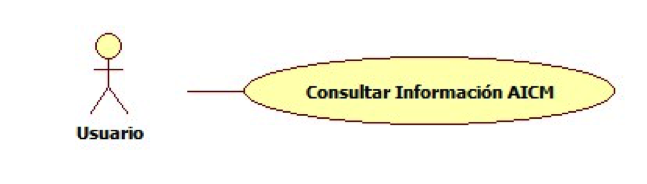
\includegraphics[width=0.9\textwidth]{Figuras/cuConsultarInformacionAICM.png}
		\rule{30em}{0.5pt}
	\caption[Diagrama de Caso de Uso Consultar Informacion AICM]{Diagrama de Caso de Uso Consultar Informacion AICM}
	\label{fig:cuConsultarInformacionAICM}
\end{figure}

\begin{longtable}{|p{2.5cm}|p{6.4cm}|p{2cm}|p{2cm}|}
	\hline
		\rowcolor[RGB]{51,153,255}{Caso de Uso}&\multicolumn{2}{c}{Consultar Información AICM}&{\textbf{CU-U-04}}\\
	\hline
		{Actores}&\multicolumn{3}{p{11.2cm}|}{Usuario}\\
	\hline
		{Tipo}&\multicolumn{3}{p{11.2cm}|}{Esencial}\\
	\hline
		{Precondición}&\multicolumn{3}{p{11.2cm}|}{El administrador ha registrado en el sistema la información del AICM.}\\
	\hline
		{Postcondición}&\multicolumn{3}{p{11.2cm}|}{El usuario tiene a su disposición la información sobre el AICM.}\\
	\hline
		{Autor}&{Vivanco Carmona Erick Rafael}&{\textbf{Fecha} 09/01/15}&{\textbf{Versión} 2.0}\\
			\hline
		{Evaluador}&{Barajas Uribe Sergio}&{\textbf{Fecha} 15/01/15}&{\textbf{Estatus} Aprobado}\\
	\hline
		{Propósito}&\multicolumn{3}{p{11.2cm}|}{Consultar la información relacionada con el AICM como es el teléfono del aeropuerto para consultar alguna duda, ubicación, servicios y página web.}\\
	\hline
		{Resumen}&\multicolumn{3}{p{11.2cm}|}{El usuario consulta la información del AICM que previamente ha sido registrada por el administrador y se encuentra disponible en la aplicación.}\\	
	\hline
	\caption[Especificación del Caso de Uso Consultar Información AICM]{Especificación del Caso de Uso Consultar Información AICM}
    	\label{tab:cuConsultarInformacionAICM}
\end{longtable}

\begin{flushleft}
	\textbf{Trayectoria Principal}\\
	\begin{enumerate}
		\item El usuario solicita la información del AICM. \hyperlink{TrayectoriaA_CU-U-04}{[Trayectoria A]}.
		\item Se despliega la información del AICM.
	\end{enumerate}
\end{flushleft}
----Fin del caso de uso

\begin{flushleft}
	\hypertarget{TrayectoriaA_CU-U-04}{}
	\textbf{Trayectoria Alternativa A}\\
	\textbf{Condición:} No existe información registrada o disponible en el sistema. \\
	\begin{enumerate}
		\item  Se notifica al turista. 
		\item Termina la operación.
	\end{enumerate}
\end{flushleft}
----Fin de Trayectoria
\subsection{Caso de Uso Gestionar Equipaje}

\begin{figure}[htbp]
	\centering
		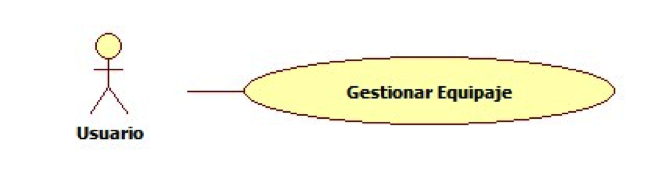
\includegraphics[width=0.9\textwidth]{Figuras/cuGestionarEquipajeU.png}
		\rule{30em}{0.5pt}
	\caption[Diagrama de Caso de Uso Gestionar Equipaje]{Diagrama de Caso de Uso Gestionar Equipaje}
	\label{fig:cuGestionarEquipajeU}
\end{figure}
\newpage
\begin{longtable}[h!]{|p{2.5cm}|p{6.4cm}|p{2cm}|p{2cm}|}
	\hline
		\rowcolor[RGB]{51,153,255}{Caso de Uso}&\multicolumn{2}{c}{Gestionar Equipaje}&{\textbf{CU-U-05}}\\
	\hline
		{Actores}&\multicolumn{3}{p{11.2cm}|}{Usuario}\\
	\hline
		{Tipo}&\multicolumn{3}{p{11.2cm}|}{Esencial}\\
	\hline
		{Precondición}&\multicolumn{3}{p{11.2cm}|}{El administrador ha registrado objetos de viaje.}\\
	\hline
		{Postcondición}&\multicolumn{3}{p{11.2cm}|}{El usuario tiene a su disposición objetos para crear lista de equipaje.}\\
	\hline
		{Autor}&{Vivanco Carmona Erick Rafael}&{\textbf{Fecha} 09/01/15}&{\textbf{Versión} 2.0}\\
			\hline
		{Evaluador}&{Barajas Uribe Sergio}&{\textbf{Fecha} 15/01/15}&{\textbf{Estatus} Aprobado}\\
	\hline
		{Propósito}&\multicolumn{3}{p{11.2cm}|}{Consultar el equipaje del usuario necesario para su viaje.}\\
	\hline
		{Resumen}&\multicolumn{3}{p{11.2cm}|}{El usuario selecciona objetos dependiendo del tipo de viaje que vaya a realizar y consulta los objetos seleccionados para su comprobación.}\\	
	\hline
		{Comentarios}&\multicolumn{3}{p{11.2cm}|}{Existen equipajes predeterminados, pero el usuario puede crear el suyo personalizado.}\\
	\hline
	\caption[Especificación del Caso de Uso Gestionar Equipaje]{Especificación del Caso de Uso Gestionar Equipaje}
    	\label{tab:cuGestionarEquipajeU}
\end{longtable}

\begin{flushleft}
	\textbf{Trayectoria Principal}\\
	\begin{enumerate}
		\item El usuario solicita crear lista de equipaje.
		\item Se solicita el nombre de la categoría de viaje.
		\item Se solicita los objetos requeridos para la lista de equipaje.
		\item Se crea la lista de equipaje.
		\item El usuario solicita verificar su equipaje.
		\item Se despliegan los objetos registrados en la lista de equipaje.
		\item El usuario verifica los objetos.
		\item El usuario edita lista de equipaje.
		\item El usuario añade objetos a la lista de equipaje.
	\end{enumerate}
\end{flushleft}
----Fin del caso de uso

\subsection{Caso de Uso Consultar Itinerario de Viaje}
\hypertarget{CU-U-06}{}

\begin{figure}[htbp]
	\centering
		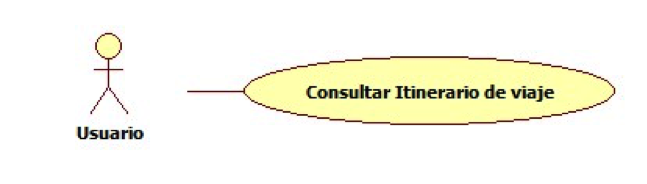
\includegraphics[width=0.9\textwidth]{Figuras/cuConsultarItinerarioViaje.png}
		\rule{30em}{0.5pt}
	\caption[Diagrama de Caso de Uso Consultar Itinerario de Viaje]{Diagrama de Caso de Uso Consultar Itinerario de Viaje}
	\label{fig:cuConsultarItinerarioViaje}
\end{figure}

\begin{longtable}{|p{2.5cm}|p{6.4cm}|p{2cm}|p{2cm}|}
	\hline
		\rowcolor[RGB]{51,153,255}{Caso de Uso}&\multicolumn{2}{c}{Consultar Itinerario de Viaje}&{\textbf{CU-U-06}}\\
	\hline
		{Actores}&\multicolumn{3}{p{11.2cm}|}{Usuario}\\
	\hline
		{Tipo}&\multicolumn{3}{p{11.2cm}|}{Esencial}\\
	\hline
		{Precondición}&\multicolumn{3}{p{11.2cm}|}{El usuario debe registrar el número de vuelo, el tipo de vuelo y la lista de actividades que realizará en el viaje.}\\
	\hline
		{Postcondición}&\multicolumn{3}{p{11.2cm}|}{El usuario tiene a su disposición la información de su vuelo, una alarma programada según el tipo viaje del usuario y un itinerario de su viaje.}\\
	\hline
		{Autor}&{Vivanco Carmona Erick Rafael}&{\textbf{Fecha} 09/01/15}&{\textbf{Versión} 2.0}\\
			\hline
		{Evaluador}&{Barajas Uribe Sergio}&{\textbf{Fecha} 15/01/15}&{\textbf{Estatus} Aprobado}\\
	\hline
		{Propósito}&\multicolumn{3}{p{11.2cm}|}{Consultar la información relacionada con su vuelo y organizar el tiempo del usuario para llegar a tiempo a su vuelo en el AICM, además de visualizar el itinerario de viaje del usuario.}\\
	\hline
		{Resumen}&\multicolumn{3}{p{11.2cm}|}{El usuario obtiene la información de su vuelo, itinerario de viaje que haya descrito previamente, se programa una alarma en el dispositivo móvil del usuario tomando en cuenta la hora de salida y el tipo de vuelo ya sea nacional la alarma se programara 3.5 horas antes e internacional 4.5 horas antes.}\\	
	\hline
		{Comentarios}&\multicolumn{3}{p{11.2cm}|}{La alarma solo podrá ser programada hasta que el usuario ingrese el tipo de vuelo, así como el itinerario que se muestre será a partir de las actividades que el usuario ingrese.}\\	
	\hline
	\caption[Especificación del Caso de Uso Consultar Itinerario de Viaje]{Especificación del Caso de Uso Consultar Itinerario de Viaje}
    	\label{tab:cuConsultarItinerarioViaje}
\end{longtable}
\newpage
\begin{flushleft}
	\textbf{Trayectoria Principal}\\
	\begin{enumerate}
		\item El usuario solicita consultar un itinerario. \hyperlink{TrayectoriaA_CU-U-06}{[Trayectoria A]}.
		\item El usuario selecciona itinerario de viaje. 
		\item El sistema solicita el  número y tipo de vuelo.
		\item El sistema valida los datos proporcionados. No permitirá avanzar si no se ingresa el número y tipo de vuelo.
		\item El sistema despliega la información de vuelo y el itinerario de viaje. \hyperlink{TrayectoriaB_CU-U-06}{[Trayectoria B]}.
		\item El sistema programa una alarma a partir de la hora de salida del vuelo y el tipo de vuelo ya se internacional con 4.5 horas antes de la salida o nacional 3.5 horas antes.
		\item El usuario solicita itinerario de viaje.
		\item	El sistema solicita una lista de actividades que el usuario gusta realizar en su viaje (itinerario).
		\item Se despliega actividades para viaje.
		\item El usuario puede gestionar su itinerario modificando, agregando o eliminando actividades.
		\item El usuario puede modificar la alarma si así lo desea.
	\end{enumerate}
\end{flushleft}
----Fin del caso de uso

\begin{flushleft}
	\hypertarget{TrayectoriaA_CU-U-06}{}
	\textbf{Trayectoria Alternativa A}\\
	\textbf{Condición:} El usuario no ha registrado itinerario\\
	\begin{enumerate}
		\item El usuario no puede consultar itinerario si aun no ha registrado alguno.
	\end{enumerate}
\end{flushleft}
----Fin de Trayectoria

\begin{flushleft}
	\hypertarget{TrayectoriaB_CU-U-06}{}
	\textbf{Trayectoria Alternativa B}\\
	\textbf{Condición:} La conexión con el servidor se pierde. \\
	\begin{enumerate}
		\item Los datos del vuelo no pueden ser cargados correctamente. 
		\item El cliente debe reintentar completar la operación en otro momento. 
		\item Volver a 2. 
	\end{enumerate}
\end{flushleft}
----Fin de Trayectoria


\subsection{Caso de Uso Consultar Ruta casa-AICM}

\begin{figure}[htbp]
	\centering
		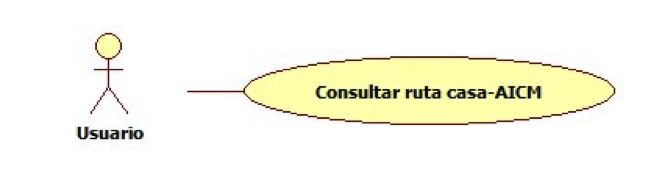
\includegraphics[width=0.9\textwidth]{Figuras/cuConsultarRutacasa-AICM.png}
		\rule{30em}{0.5pt}
	\caption[Diagrama de Caso de Uso Consultar Ruta casa-AICM]{Diagrama de Caso de Uso Consultar Ruta casa-AICM}
	\label{fig:cuConsultarRutacasa-AICM}
\end{figure}

\begin{longtable}{|p{2.5cm}|p{6.4cm}|p{2cm}|p{2cm}|}
	\hline
		\rowcolor[RGB]{51,153,255}{Caso de Uso}&\multicolumn{2}{c}{Consultar Ruta casa-AICM}&{\textbf{CU-U-07}}\\
	\hline
		{Actores}&\multicolumn{3}{p{11.2cm}|}{Usuario}\\
	\hline
		{Tipo}&\multicolumn{3}{p{11.2cm}|}{Esencial}\\
	\hline
		{Precondición}&\multicolumn{3}{p{11.2cm}|}{El usuario deberá estar conectado a una red de internet para generar la ruta de su origen al aeropuerto.}\\
	\hline
		{Postcondición}&\multicolumn{3}{p{11.2cm}|}{Se obtiene la ruta desde el punto de origen hacia el AICM.}\\
	\hline
		{Autor}&{Vivanco Carmona Erick Rafael}&{\textbf{Fecha} 09/01/15}&{\textbf{Versión} 2.0}\\
			\hline
		{Evaluador}&{Barajas Uribe Sergio}&{\textbf{Fecha} 15/01/15}&{\textbf{Estatus} Aprobado}\\
	\hline
		{Propósito}&\multicolumn{3}{p{11.2cm}|}{Obtener la ruta desde el origen del usuario al AICM.}\\
	\hline
		{Resumen}&\multicolumn{3}{p{11.2cm}|}{El usuario desea conocer cuál es la ruta para llegar al AICM desde su punto de origen. Por lo tanto, solicita dicha función al sistema, el sistema obtiene la ubicación actual del usuario y  genera la ruta hacia el AICM.}\\	
	\hline
		{Comentarios}&\multicolumn{3}{p{11.2cm}|}{El usuario debe estar conecta a una red para generar la ruta.}\\
	\hline
	\caption[Especificación del Caso de Uso Consultar Ruta casa-AICM]{Especificación del Caso de Uso Consultar Ruta casa-AICM}
    	\label{tab:cuConsultarRutacasa-AICM}
\end{longtable}

\begin{flushleft}
	\textbf{Trayectoria Principal}\\
	\begin{enumerate}
		\item El usuario solicita generar una nueva ruta casa-AICM. \hyperlink{TrayectoriaA_CU-U-07}{[Trayectoria A]}.
		\item Se obtiene la ubicación actual del usuario y se genera la ruta hacia el AICM.
		\item El usuario tiene a su disposición la ruta sugerida por el sistema para llegar desde su ubicación actual hacia el AICM.
	\end{enumerate}
\end{flushleft}
----Fin del caso de uso

\begin{flushleft}
	\hypertarget{TrayectoriaA_CU-U-07}{}
	\textbf{Trayectoria Alternativa A}\\
	\textbf{Condición:} No existe conexión con una red para generar la ruta. \\
	\begin{enumerate}
		\item Se solicita al usuario que se conecte a una red para generar la ruta. 
		\item Volver a 1.
	\end{enumerate}
\end{flushleft}
----Fin de Trayectoria

\subsection{Caso de Uso Ubicar en AICM}

\begin{figure}[htbp]
	\centering
		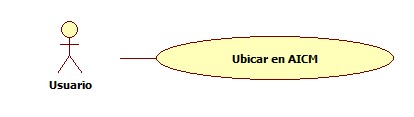
\includegraphics[width=0.9\textwidth]{Figuras/cuUbicarAICM.jpg}
		\rule{30em}{0.5pt}
	\caption[Diagrama de Caso de Uso Ubicar en AICM]{Diagrama de Caso de Uso Ubicar en AICM}
	\label{fig:cuUbicarAICM}
\end{figure}
\newpage
\begin{longtable}{|p{2.5cm}|p{6.4cm}|p{2cm}|p{2cm}|}
	\hline
		\rowcolor[RGB]{51,153,255}{Caso de Uso}&\multicolumn{2}{c}{Ubicar en AICM}&{\textbf{CU-U-08}}\\
	\hline
		{Actores}&\multicolumn{3}{p{11.2cm}|}{Usuario}\\
	\hline
		{Tipo}&\multicolumn{3}{p{11.2cm}|}{Esencial}\\
	\hline
		{Precondición}&\multicolumn{3}{p{11.2cm}|}{El sistema deberá estar entrenado en el AICM, y las salas de abordaje estarán previamente registradas.}\\
	\hline
		{Postcondición}&\multicolumn{3}{p{11.2cm}|}{Se obtiene la localización del usuario dentro del AICM.}\\
	\hline
		{Autor}&{Vivanco Carmona Erick Rafael}&{\textbf{Fecha} 09/01/15}&{\textbf{Versión} 2.0}\\
			\hline
		{Evaluador}&{Barajas Uribe Sergio}&{\textbf{Fecha} 15/01/15}&{\textbf{Estatus} Aprobado}\\
	\hline
		{Propósito}&\multicolumn{3}{p{11.2cm}|}{Obtener la ubicación del usuario dentro del AICM mediante el magnetómetro integrado en el dispositivo móvil, así como localizar la sala de abordaje y servicios en el AICM. }\\
	\hline
		{Resumen}&\multicolumn{3}{p{11.2cm}|}{El usuario solicita explorar el AICM, el sistema despliega la sala de abordaje que el usuario haya proporcionado y visualiza los servicios en el interior del AICM.}\\	
	\hline
		{Comentarios}&\multicolumn{3}{p{11.2cm}|}{El sistema deberá estar entrenado, de lo contrario, la ubicación será ineficiente.}\\
	\hline
	\caption[Especificación del Caso de Uso Ubicar en AICM]{Especificación del Caso de Uso Ubicar en AICM}
    	\label{tab:cuUbicarAICM}
\end{longtable}

\begin{flushleft}
	\textbf{Trayectoria Principal}\\
	\begin{enumerate}
		\item El turista solicita localizarse en el AICM.
		\item El sistema despliega un mapa del AICM donde se puede ubicar al usuario así como su sala de abordaje y servicios disponibles.
		\item El usuario tiene a su disposición el mapa el cual le mostrar su ubicación actual y permitirá desplazarse con mayor facilidad dentro del AICM.
	\end{enumerate}
\end{flushleft}
----Fin del caso de uso
\newpage
\subsection{Caso de Uso Consultar Información de Vuelo}

\begin{figure}[htbp]
	\centering
		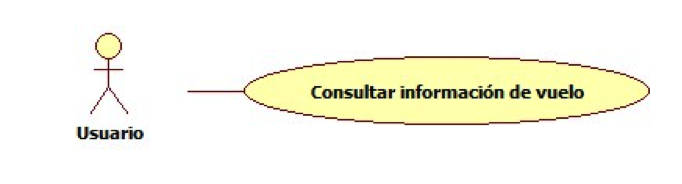
\includegraphics[width=0.9\textwidth]{Figuras/cuConsultarInformacionVuelo.png}
		\rule{30em}{0.5pt}
	\caption[Diagrama de Caso de Uso Consultar Información de Vuelo]{Diagrama de Caso de Uso Consultar Información de Vuelo}
	\label{fig:cuConsultarInformacionVuelo}
\end{figure}

\begin{longtable}{|p{2.5cm}|p{6.4cm}|p{2cm}|p{2cm}|}
	\hline
		\rowcolor[RGB]{51,153,255}{Caso de Uso}&\multicolumn{2}{c}{Consultar Información de Vuelo}&{\textbf{CU-U-09}}\\
	\hline
		{Actores}&\multicolumn{3}{p{11.2cm}|}{Usuario}\\
	\hline
		{Tipo}&\multicolumn{3}{p{11.2cm}|}{Esencial}\\
	\hline
		{Precondición}&\multicolumn{3}{p{11.2cm}|}{	El usuario ha registrado su número de vuelo.}\\
	\hline
		{Postcondición}&\multicolumn{3}{p{11.2cm}|}{El usuario tendrá a su disposición la información de su vuelo.}\\
	\hline
		{Autor}&{Vivanco Carmona Erick Rafael}&{\textbf{Fecha} 09/01/15}&{\textbf{Versión} 2.0}\\
			\hline
		{Evaluador}&{Barajas Uribe Sergio}&{\textbf{Fecha} 15/01/15}&{\textbf{Estatus} Aprobado}\\
	\hline
		{Propósito}&\multicolumn{3}{p{11.2cm}|}{Consultar la información relacionada con el vuelo del usuario.}\\
	\hline
		{Resumen}&\multicolumn{3}{p{11.2cm}|}{El usuario solicita la información relacionada con un número de vuelo previamente registrado. Una vez registrado un número de vuelo el sistema proporciona el estado del vuelo, la ciudad de origen y destino, hora de salida y llegada, fecha y terminal, así como el seguimiento del vuelo ya que el usuario se encuentra viajando en el avión.}\\	
	\hline
	\caption[Especificación del Caso de Uso Consultar Información de Vuelo]{Especificación del Caso de Uso Consultar Información de Vuelo}
    	\label{tab:cuConsultarInformacionVuelo}
\end{longtable}

\begin{flushleft}
	\textbf{Trayectoria Principal}\\
	\begin{enumerate}
		\item El usuario solicita la información de vuelo. \hyperlink{TrayectoriaA_CU-U-09}{[Trayectoria A]}.
		\item El sistema solicita el número de vuelo.
		\item El sistema despliega la información relacionada con el número de vuelo. \hyperlink{TrayectoriaB_CU-U-09}{[Trayectoria B]} \hyperlink{TrayectoriaC_CU-U-09}{[Trayectoria C]}.
		\item El usuario tiene a su disposición la información referente a su vuelo.
		\item El usuario selecciona la actividad de seguimiento de vuelo.
		\item	Se despliega un mapa donde se muestra la posición actual del avión.
	\end{enumerate}
\end{flushleft}
----Fin del caso de uso

\begin{flushleft}
	\hypertarget{TrayectoriaA_CU-U-09}{}
	\textbf{Trayectoria Alternativa A}\\
	\textbf{Condición:} Solicitar información del vuelo \\
	\begin{enumerate}
		\item El sistema valida si el número de vuelo se ingreso en el \hyperlink{CU-U-06}{[CU-U-06]}. 
		\item Se notifica al usuario si existe un número de vuelo registrado.
		\item Se continúa con el proceso.
	\end{enumerate}
\end{flushleft}
----Fin de Trayectoria

\begin{flushleft}
	\hypertarget{TrayectoriaB_CU-U-09}{}
	\textbf{Trayectoria Alternativa B}\\
	\textbf{Condición:} La conexión con el servidor se pierde. \\
	\begin{enumerate}
		\item Los datos del vuelo no pueden ser cargados correctamente. 
		\item El cliente debe reintentar completar la operación en otro momento. 
		\item Volver a 1.
	\end{enumerate}
\end{flushleft}
----Fin de Trayectoria

\begin{flushleft}
	\hypertarget{TrayectoriaC_CU-U-09}{}
	\textbf{Trayectoria Alternativa C}\\
	\textbf{Condición:} La conexión con la red se pierde. \\
	\begin{enumerate}
		\item El mapa no se puede mostrar correctamente. 
		\item El cliente debe reintentar completar la operación en otro momento. 
		\item Volver a 1.
	\end{enumerate}
\end{flushleft}
----Fin de Trayectoria